\newday{Planos Fatoriais}

Em estatística, um plano fatorial (também conhecido como ``\emph{factorial design}'', em inglês) investiga a forma como vários fatores influenciam um resultado específico, designado por variável de resposta.
Cada fator é testado em valores distintos, ou níveis, e a experiência inclui todas as combinações possíveis destes níveis em todos os fatores.
Esta abordagem abrangente permite aos investigadores ver como não só como cada fator influencia individualmente a variável de resposta, mas também como os fatores interagem entre si e se influenciam mutuamente.

\begin{marginfigure}
    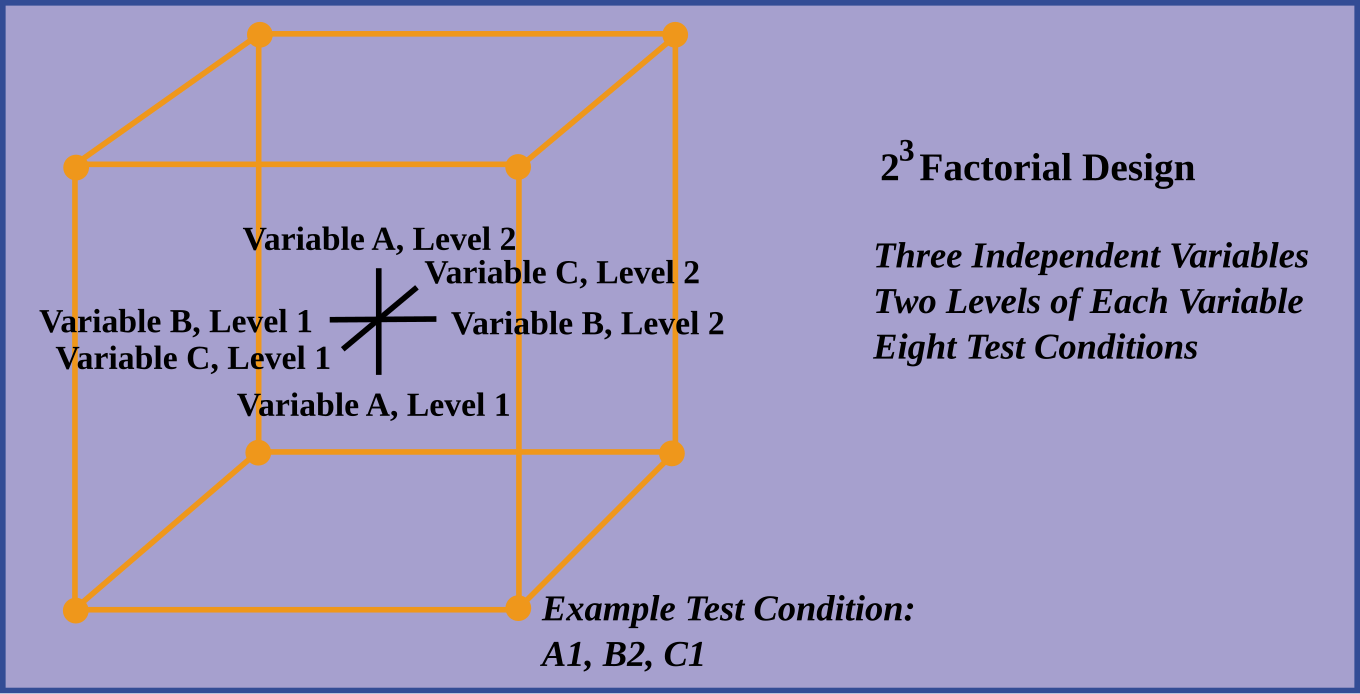
\includegraphics[width=\linewidth]{figures/plano fatorial exemplo}
    \caption{Gráfico de cubos para o plano fatorial.}
    \label{fig:plano_fatorial_exemplo}
\end{marginfigure}

Os planos fatoriais podem ser simplificados se apenas se utilizar dois níveis de variação para cada fator, um nível inferior e um nível superior. 
Por exemplo, um plano fatorial $2\times2$ tem dois fatores, cada um com dois níveis de variação, resultando em quatro combinações únicas que serão testadas.
A interação entre estes fatores é frequentemente o resultado mais importante, mesmo quando os fatores individuais também têm um efeito.

Foram realizados dois planos fatoriais, um plano fatorial para a lixiviação com Tioureia e um plano fatorial para a lixiviação com Citrato.
Para a lixiviação com Tioureia foi elaborado um plano fatorial com 4 fatores\sidenote{Ou seja, 16 combinações, que foram reduzidas a 1/2, resultando em 8 combinações.} e variação de dois níveis.
Para a lixiviação com Citrato foi elaborado um plano fatorial com 6 fatores\sidenote{Ou seja, 64 combinações, que foram reduzidas a 1/8, resultando em 8 combinações.} e variação de dois níveis.

A Tabela~\ref{tab:plano_fatorial_tioureia1} mostra os fatores e os níveis de variação para o plano fatorial com Tioureia.

\begin{table}
  \caption{Fatores e níveis de variação para a Tioureia.}\label{tab:plano_fatorial_tioureia1}
  \begin{tabularx}{\textwidth}{@{}lCC@{}}
    \toprule
    \textbf{Fatores} & \textbf{Nível Inferior} & \textbf{Nível Superior} \\ \midrule
    A - \ce{CH4N2S} (g/kg) & 200 & 300 \\
    B - \ce{Fe(SO4)3} (g/kg) & 1 & 2 \\
    C - Temperatura (\graus{}) & 20 & 60 \\
    D - Tempo (h) & 4 & 6 \\ \bottomrule
  \end{tabularx}
\end{table}

A Tabela~\ref{tab:plano_fatorial_citrato1} mostra os fatores e os níveis de variação para o plano fatorial com Tioureia.

\begin{table}
  \caption{Fatores e níveis de variação para o Citrato.}\label{tab:plano_fatorial_citrato1}
  \begin{tabularx}{\textwidth}{@{}lCC@{}}
    \toprule
    \textbf{Fatores} & \textbf{Nível Inferior} & \textbf{Nível Superior} \\ \midrule
    A - \ce{Na2S2O3} (mol/L) & 0,1 & 0,3 \\
    B - \ce{CuSO4} (mol/L) & 0,1 & 0,2 \\
    C - \ce{Na3C6H5O7} (mol/L) & 0,1 & 0,3 \\
    D - Temperatura (\graus{}) & 50 & 70 \\
    E - Tempo (h) & 7 & 9 \\
    F - pH & 7 & 11 \\ \bottomrule
  \end{tabularx}
\end{table}

Em ambos os planos fatoriais, a quantidade de minério a ser lixiviada e a relação sólido líquido mantiveram-se constantes, sendo 100~g e L/S = 1/5, respetivamente.

\begin{table}
  \caption{Plano fatorial com Tioureia.}
  \begin{tabularx}{\textwidth}{@{}>{\bfseries}CCCCC@{}}
    \toprule
    \textbf{OrdemPad} & \textbf{A} & \textbf{B} & \textbf{C} & \textbf{D} \\ \midrule
    2 & 1 & -1 & -1 & 1 \\
    7 & -1 & 1 & 1 & -1 \\
    4 & 1 & 1 & -1 & -1 \\
    3 & -1 & 1 & -1 & 1 \\
    1 & -1 & -1 & -1 & -1 \\
    8 & 1 & 1 & 1 & 1 \\
    6 & 1 & -1 & 1 & -1 \\
    5 & -1 & -1 & 1 & 1 \\ \bottomrule
  \end{tabularx}
\end{table}

Ou seja, foram realizados 8 ensaios de lixiviação.
